% !TeX root = ../../thesis.tex
\chapter{Fabrication and Characterization: From Perovskite Films to Photodetectors}\label{ch:material_properties}


\section{Perovskite deposition via thermal co-evaporation}

\begin{itemize}
    \item Visual icon of the co-evaporation chamber and explanation of parts + add icon of the substrate holder
    \item Sources and calibration of tooling factor - evaporation rates through spectroscopic ellipsometry (add plots that show the fitting and the average)
    \item Selection of co-evaporation rate/ratio and why
\end{itemize}

\subsection{Annealing effect on perovskite properties}

\begin{itemize}
    \item Characterization of as-deposited and annealed films via AFM, SEM, SSPL, TRPL, aborptance/reflectance measurements, XPS/UPS
    \item In situ characterization through in situ, temperature dependent GIWAXS, phase identification, phase transition identification, 0-D phase emergence, crystallite size etc
\end{itemize}

\section{Device Fabrication}

\begin{itemize}
    \item Options for transport layers, deposition techniques and associated challenges, NiO always below the perovskite layer, explanation of NiO annealing effect on the conductivity of the perovskite layer
    \item Option for substrates (ITO - PIX), same stack, different source of light, masks and contacts
    \item Most important characterization for devices, specifications of figures of merit that are followed in this thesis, considerations on yield and statistical importance of the presented results
    \item (From Valdimir's thesis) Variations in the forward bias regime, device performance is very sensitive to small variations in resistance, it is not major focus in the work presented
\end{itemize}

\subsection{Baseline performance on Glass and Silicon substrates}

\begin{itemize}
    \item Comparison of JVs and EQE between glass/ITO and PIX 
    \item Explanation of the higher resistivity of the PIX substrates through the TEM submitted samples
    \item Proof of the high-temperature stability of the stack through annealing of the complete PIX stack post-depositions
    \item Only possible to evaluate for PIX and not for Al, since it will diffuse in the stack 
\end{itemize}

\section{Impact of Deposition Conditions}

\begin{itemize}
    \item Part on defect tolerance of the perovskite layer and its implications on the tolerance against changes in the device characteristics by changing deposition consitions
    \item Impact of deposition rate, ratio between precursors, annealing duration
    \item Exploration of 3-source evaporation of CsPbI2Br films and the problems with pinholes and shunts in device performance. 
\end{itemize}


An illustration of the deposition chamber is provided in Figure~\ref{fig:deposition_chamber}. Two diametrically opposed sources are loaded with CsBr and PbI2 powders, respectively. Two separate quartz monitors are used to monitor the deposition rate of each source. The quartz crystals are individually calibrated by depositing each material on its own and later measuring its thickness using spectroscopic ellipsometry. Then, the tooling factor is corrected using the equation TFfinal = Tfinitial thickness(estimated)/thickness(real). 




% % Some dummy code show how to include images.
\begin{figure}
  \centering
  \medskip
  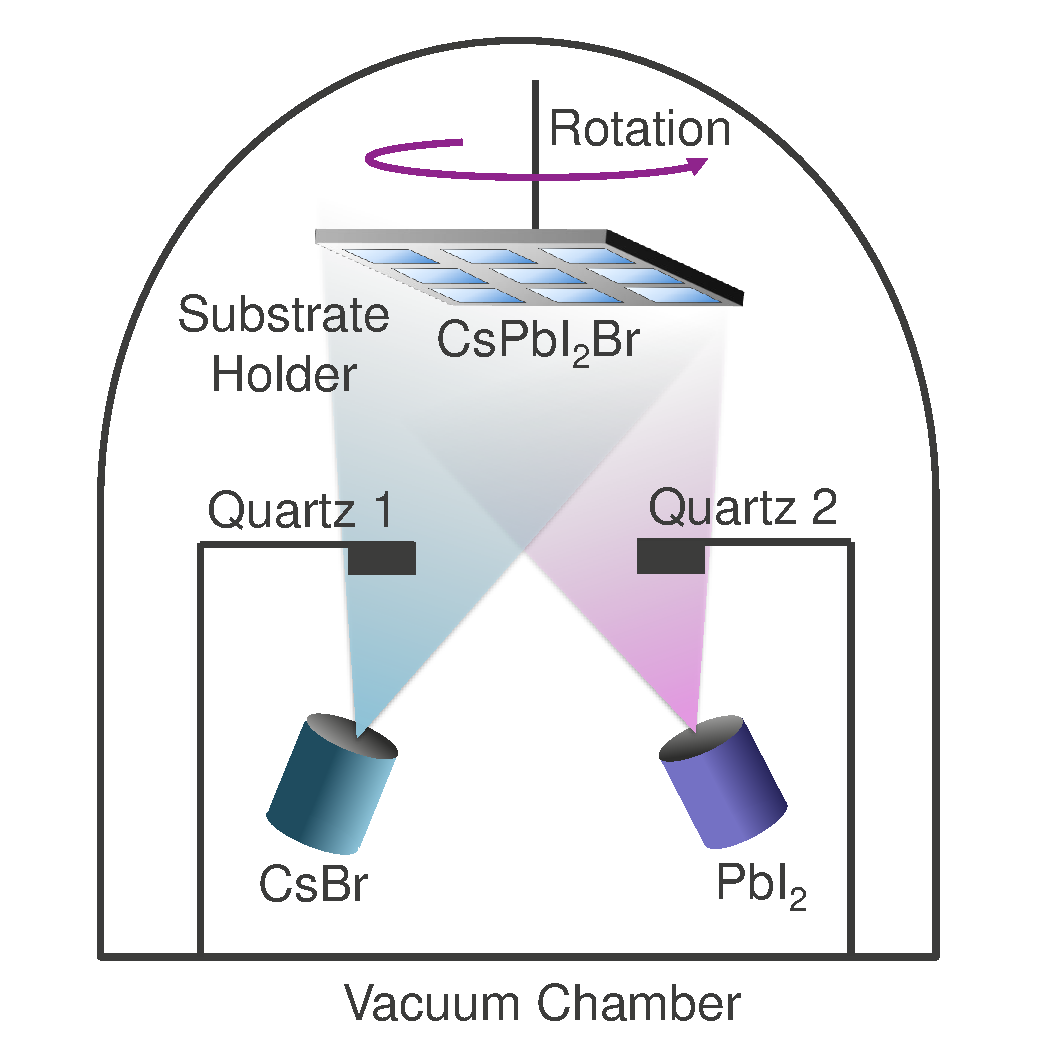
\includegraphics[width=.5\textwidth]{chapters/material_properties/images/Chamber.pdf}
  \caption[Short caption for Table of Figures]{Illustration of the deposition chamber. Two diametrically opposed sources are used for CsBr and PbI2.}
  \label{fig:deposition_chamber}
\end{figure}


\begin{figure}[htbp]
    \centering
    % First row
    \begin{subfigure}[t]{0.45\textwidth}
        \centering
        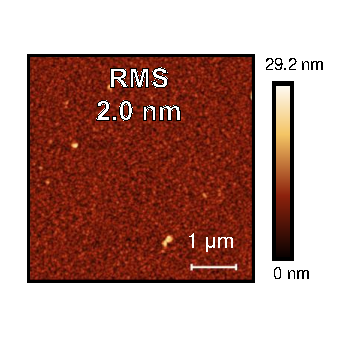
\includegraphics[width=\textwidth]{chapters/material_properties/images/AFM_before.pdf} % Replace with your image file
        \caption*{(a)}
    \end{subfigure}
    \hfill
    \begin{subfigure}[t]{0.45\textwidth}
        \centering
        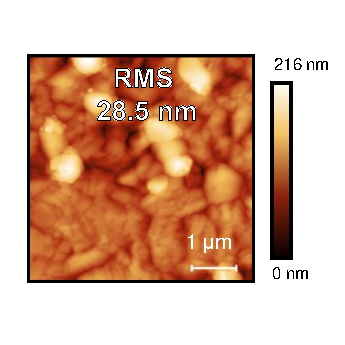
\includegraphics[width=\textwidth]{chapters/material_properties/images/AFM_after.pdf} % Replace with your image file
        \caption*{(b)}
    \end{subfigure}

    \vspace{1em} % Space between rows

    % Second row
    \begin{subfigure}[t]{0.4\textwidth}
        \centering
        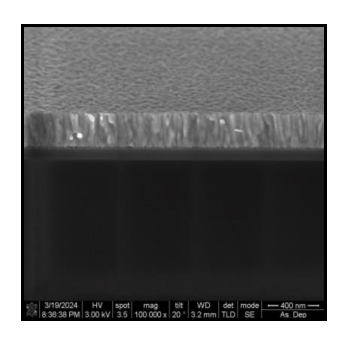
\includegraphics[width=\textwidth]{chapters/material_properties/images/SEM_Before.pdf} % Replace with your image file
        \caption*{(c)}
    \end{subfigure}
    \hfill
    \begin{subfigure}[t]{0.4\textwidth}
        \centering
        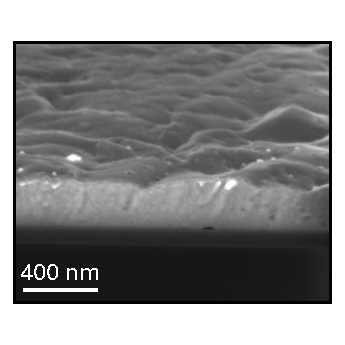
\includegraphics[width=\textwidth]{chapters/material_properties/images/SEM_After.pdf} % Replace with your image file
        \caption*{(d)}
    \end{subfigure}
    \caption{AFM and SEM iamges for an as-deposited and annealed perovskite sample.}
\end{figure}


\begin{figure}[htbp]
    \centering
    % First row
    \begin{subfigure}[t]{0.45\textwidth}
        \centering
        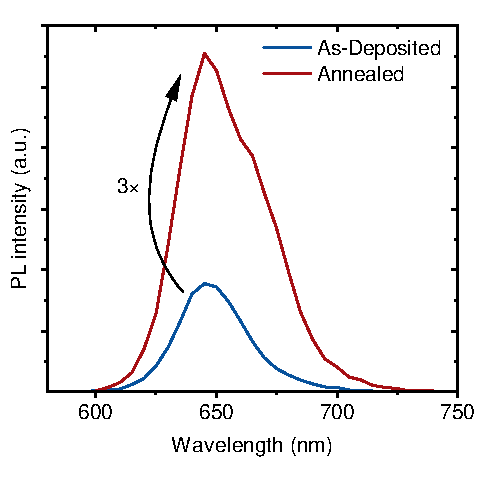
\includegraphics[width=\textwidth]{chapters/material_properties/images/SSPL.pdf} % Replace with your image file
        \caption*{(a)}
    \end{subfigure}
    \hfill
    \begin{subfigure}[t]{0.45\textwidth}
        \centering
        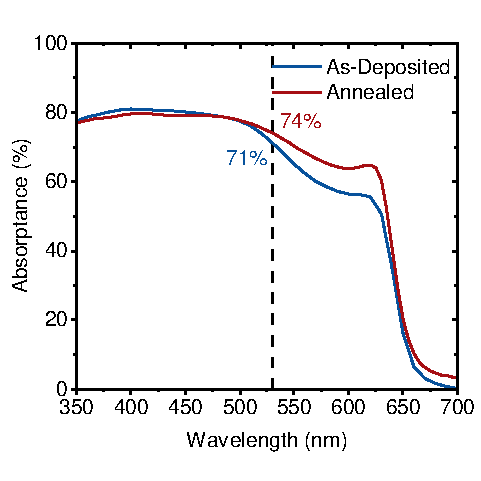
\includegraphics[width=\textwidth]{chapters/material_properties/images/Absorptance.pdf} % Replace with your image file
        \caption*{(b)}
    \end{subfigure}

    \vspace{1em} % Space between rows

    % Second row
    \begin{subfigure}[t]{0.45\textwidth}
        \centering
        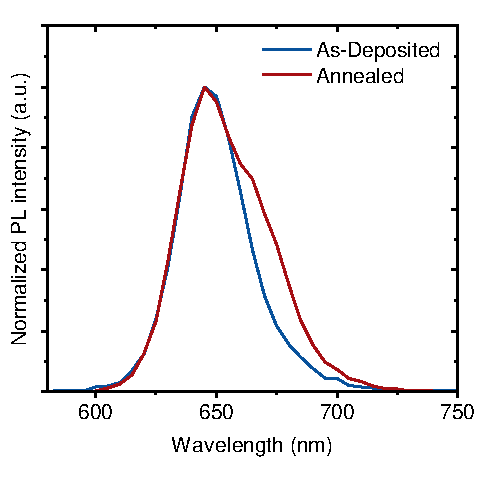
\includegraphics[width=\textwidth]{chapters/material_properties/images/SSPL_norm.pdf} % Replace with your image file
        \caption*{(c)}
    \end{subfigure}
    \hfill
    \begin{subfigure}[t]{0.45\textwidth}
        \centering
        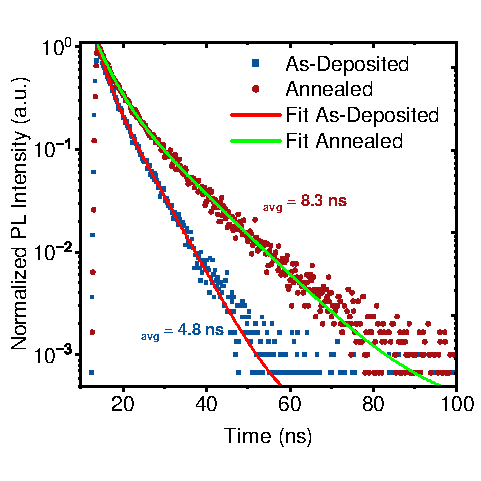
\includegraphics[width=\textwidth]{chapters/material_properties/images/TRPL_norm_double - Copy.pdf} % Replace with your image file
        \caption*{(d)}
    \end{subfigure}
    \caption{SSPL, TRPL, and absorptance for the an As-Deposited and an Annealed perovskite sample.}
\end{figure}


% % Some dummy code show how to include images.
\begin{figure}
  \centering
  \medskip
  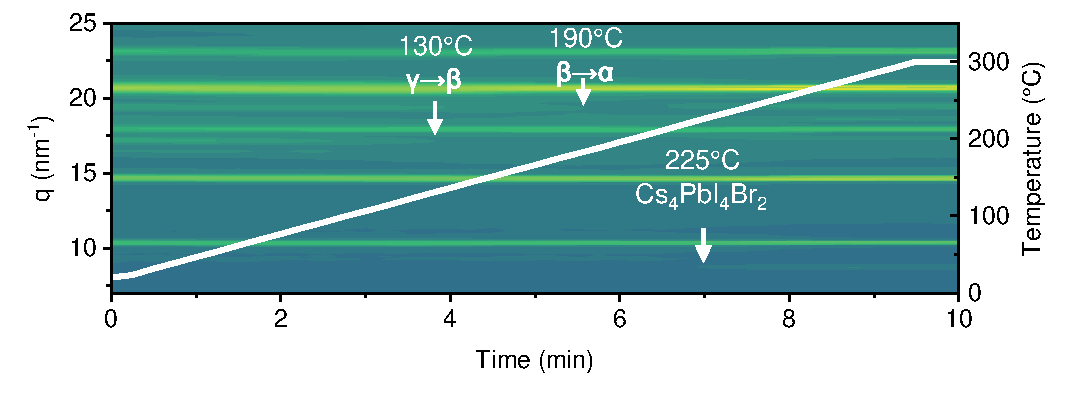
\includegraphics[width=\textwidth]{chapters/material_properties/images/GIWAXS_In_Situ.pdf}
  \caption[Short caption for Table of Figures]{In Situ GIWAXS}
  \label{}
\end{figure}

\begin{figure}
  \centering
  \medskip
  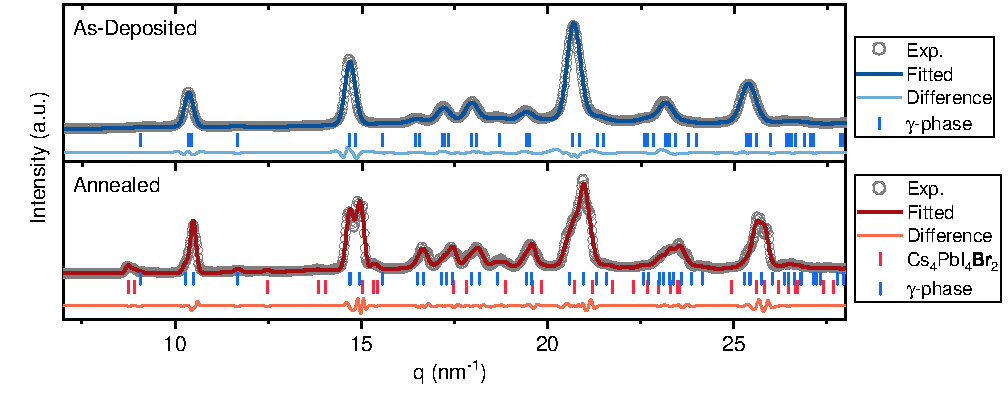
\includegraphics[width=\textwidth]{chapters/material_properties/images/GIWAXS_Before_After.pdf}
  \caption[Short caption for Table of Figures]{In Situ GIWAXS}
  \label{}
\end{figure}

\begin{figure}[htbp]
    \centering
    % First plot
    \begin{subfigure}[t]{0.49\textwidth} % Adjust width as needed
        \centering
        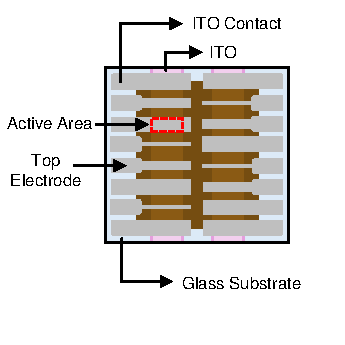
\includegraphics[width=\textwidth]{chapters/material_properties/images/Glass_Substrate.pdf} % Replace with your image
        \caption{Description for subplot (a).}
        \label{fig:sub-a}
    \end{subfigure}
    \hfill % Space between the two plots
    % Second plot
    \begin{subfigure}[t]{0.49\textwidth} % Adjust width as needed
        \centering
        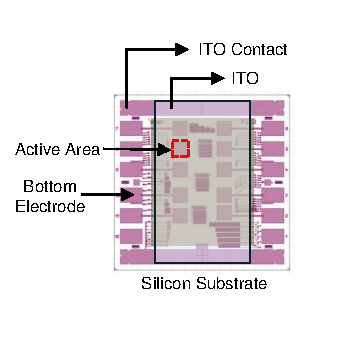
\includegraphics[width=\textwidth]{chapters/material_properties/images/PIX_Substrate.pdf} % Replace with your image
        \caption{Description for subplot (b).}
        \label{fig:sub-b}
    \end{subfigure}

    % Caption for the whole figure
    \caption{Comparison of experimentally measured and simulated Absorptance and Reflectance for the As-Deoisted and Annealed perovskite state.}
    \label{fig:1x2plot}
\end{figure}

\begin{figure}[htbp]
    \centering
    % First plot
    \begin{subfigure}[t]{0.49\textwidth} % Adjust width as needed
        \centering
        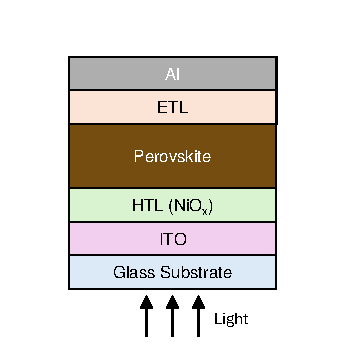
\includegraphics[width=\textwidth]{chapters/material_properties/images/Glass_Stack.pdf} % Replace with your image
        \caption{Description for subplot (a).}
        \label{fig:sub-a}
    \end{subfigure}
    \hfill % Space between the two plots
    % Second plot
    \begin{subfigure}[t]{0.49\textwidth} % Adjust width as needed
        \centering
        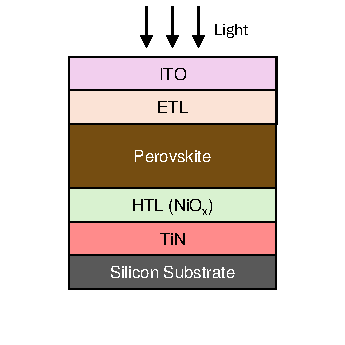
\includegraphics[width=\textwidth]{chapters/material_properties/images/PIX_Stack.pdf} % Replace with your image
        \caption{Description for subplot (b).}
        \label{fig:sub-b}
    \end{subfigure}

    % Caption for the whole figure
    \caption{Comparison of experimentally measured and simulated Absorptance and Reflectance for the As-Deoisted and Annealed perovskite state.}
    \label{fig:1x2plot}
\end{figure}

\begin{figure}[h!]
    \centering
    % First row: Two figures
    \begin{minipage}{0.48\textwidth}
        \centering
        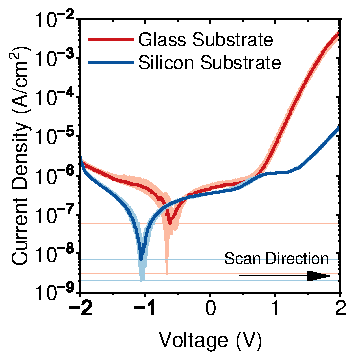
\includegraphics[width=\textwidth]{chapters/material_properties/images/JV_PIX_Glass.pdf} % Replace with your file
        \caption{Figure 1 Caption}
        \label{fig:figure1}
    \end{minipage}
    \hfill
    \begin{minipage}{0.48\textwidth}
        \centering
        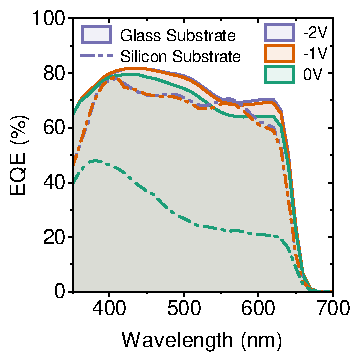
\includegraphics[width=\textwidth]{chapters/material_properties/images/EQE_fnm_PIX_Glass.pdf} % Replace with your file
        \caption{Figure 2 Caption}
        \label{fig:figure2}
    \end{minipage}

    % Second row: One figure
    \vspace{1em} % Adjust vertical space
    \begin{minipage}{0.48\textwidth}
        \centering
        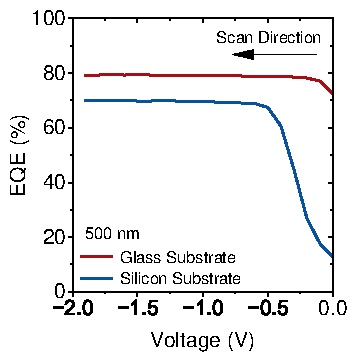
\includegraphics[width=\textwidth]{chapters/material_properties/images/EQE_fV_PIX_Glass.pdf} % Replace with your file
        \caption{Figure 3 Caption}
        \label{fig:figure3}
    \end{minipage}
\end{figure}


\begin{figure}[htbp]
    \centering
    % First row
    \begin{subfigure}[t]{0.49\textwidth}
        \centering
        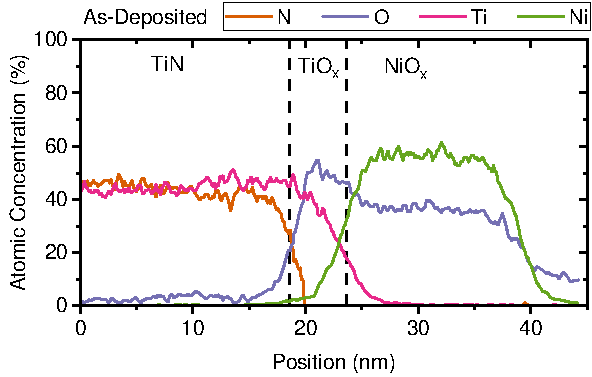
\includegraphics[width=\textwidth]{chapters/material_properties/images/TEM_As_Dep.pdf} % Replace with your image file
        \caption*{(a)}
    \end{subfigure}
    \hfill
    \begin{subfigure}[t]{0.49\textwidth}
        \centering
        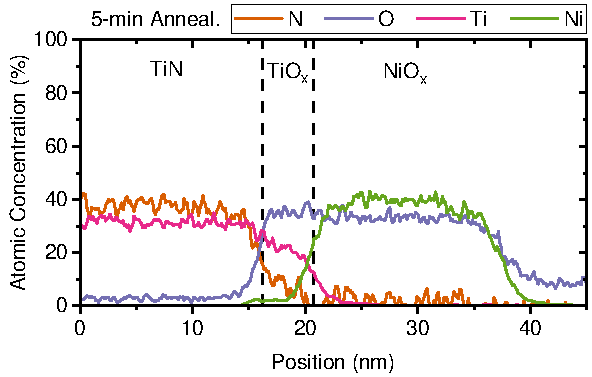
\includegraphics[width=\textwidth]{chapters/material_properties/images/TEM_5_min.pdf} % Replace with your image file
        \caption*{(b)}
    \end{subfigure}

    \vspace{1em} % Space between rows

    % Second row
    \begin{subfigure}[t]{0.49\textwidth}
        \centering
        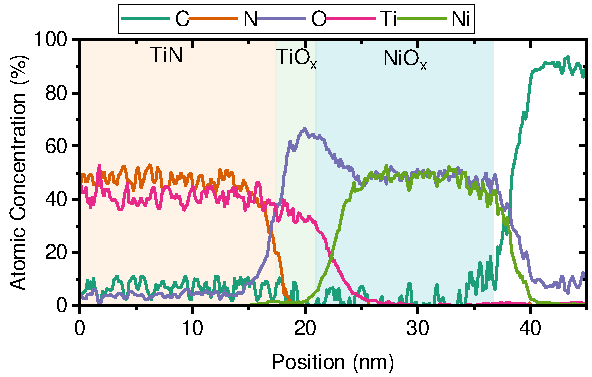
\includegraphics[width=\textwidth]{chapters/material_properties/images/TEM_30_min.pdf} % Replace with your image file
        \caption*{(c)}
    \end{subfigure}
    \hfill
    \begin{subfigure}[t]{0.49\textwidth}
        \centering
        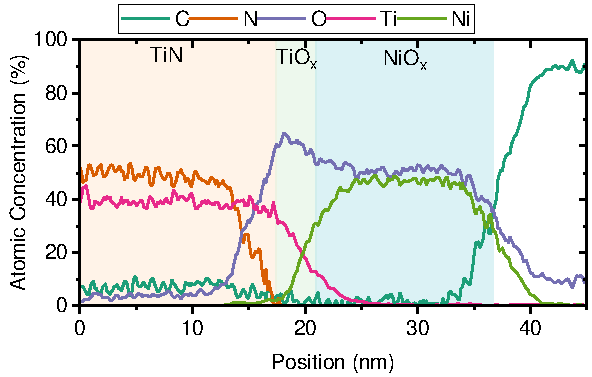
\includegraphics[width=\textwidth]{chapters/material_properties/images/TEM_60_min.pdf} % Replace with your image file
        \caption*{(d)}
    \end{subfigure}
    \caption{TEM of TiN - NiOx interface and emergence of TiOx at the interface.}
\end{figure}




%%%%%%%%%%%%%%%%%%%%%%%%%%%%%%%%%%%%%%%%%%%%%%%%%%
% Keep the following \cleardoublepage at the end of this file, 
% otherwise \includeonly includes empty pages.
\cleardoublepage

